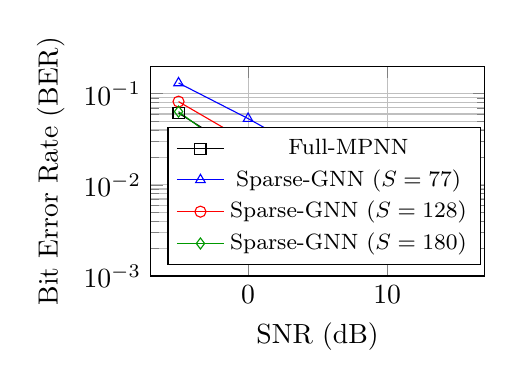
\begin{tikzpicture}
\begin{semilogyaxis}[
    xlabel={SNR (dB)},
    ylabel={Bit Error Rate (BER)},
    grid=both,
    legend style={at={(0.05,0.05)}, anchor=south west, font=\footnotesize},
    mark options={solid},
    width=0.48\textwidth,
    height=0.35\textwidth,
    ymin=1e-3, ymax=2e-1
]
\addplot[color=black, mark=square] coordinates {(-5, 0.061312) (0, 0.020531) (5, 0.010219) (10, 0.007844) (15, 0.008031)};
\addlegendentry{Full-MPNN}
\addplot[color=blue, mark=triangle] coordinates {(-5, 0.131281) (0, 0.053437) (5, 0.020094) (10, 0.011031) (15, 0.011219)};
\addlegendentry{Sparse-GNN ($S=77$)}
\addplot[color=red, mark=o] coordinates {(-5, 0.082000) (0, 0.029562) (5, 0.013469) (10, 0.010937) (15, 0.009250)};
\addlegendentry{Sparse-GNN ($S=128$)}
\addplot[color=green!60!black, mark=diamond] coordinates {(-5, 0.063687) (0, 0.017469) (5, 0.005625) (10, 0.003969) (15, 0.003812)};
\addlegendentry{Sparse-GNN ($S=180$)}
\end{semilogyaxis}
\end{tikzpicture}